\documentclass[12pt]{report}

\usepackage{amssymb,amsmath}

\usepackage[utf8]{inputenc}
\usepackage{graphicx, graphics, epsfig}
\usepackage{epstopdf}
\usepackage{ifpdf}   
\usepackage{amsfonts}
\usepackage{mathrsfs}
\usepackage[english,russian]{babel}
%\usepackage[pdftex,unicode]{hyperref}
%\usepackage[noend]{algorithm}
%\usepackage[noend]{algpseudocode}
\usepackage{multicol}
\textheight=24cm
\textwidth=16cm
\oddsidemargin=0pt
\topmargin=-1.5cm
\parindent=24pt
\parskip=0pt
\tolerance=2000
\flushbottom
\def\baselinestretch{1.2} 

\author{Вишневский~Валерий~Викторович}

\begin{document}
\newcommand{\Var}{\mathsf{var}}
\newcommand{\Erf}{\mathsf{erf}}
%\thispagestyle{empty}

Схема следующая: для всех 24 файлов(12 из Контроля, 12 из Группы без гиппокампа) ищутся паттерны.
Получается 24 набора паттернов. потом для каждого набора файла $x$, для каждого паттерна из этого набора, смотрим как входит этот
паттерн в данные из файла $y$.
Возможно несколько способов подсчета числа <<матчей>> паттернов из файла $x$ в файле $y$:
\begin{itemize}
 \item 
для каждого паттерна из $x$, если он(паттерн) длиннее $MinPat$, добавляем к числу матчей {\em число встреч }
этого паттерна в файле $y$(frequent).
\item
для каждого паттерна из $x$, если он(паттерн) длиннее $MinPat$, добавляем к числу матчей {\em единичку}, если
этот паттерна встречается в $y$(boolean).
\end{itemize}
Тоесть надо сделать 2 выбора:
минимальная длинна паттерна; добавлять число встреч паттерна, или 1, если true, и 0 если false.

\begin{figure}[h]
\noindent\centering{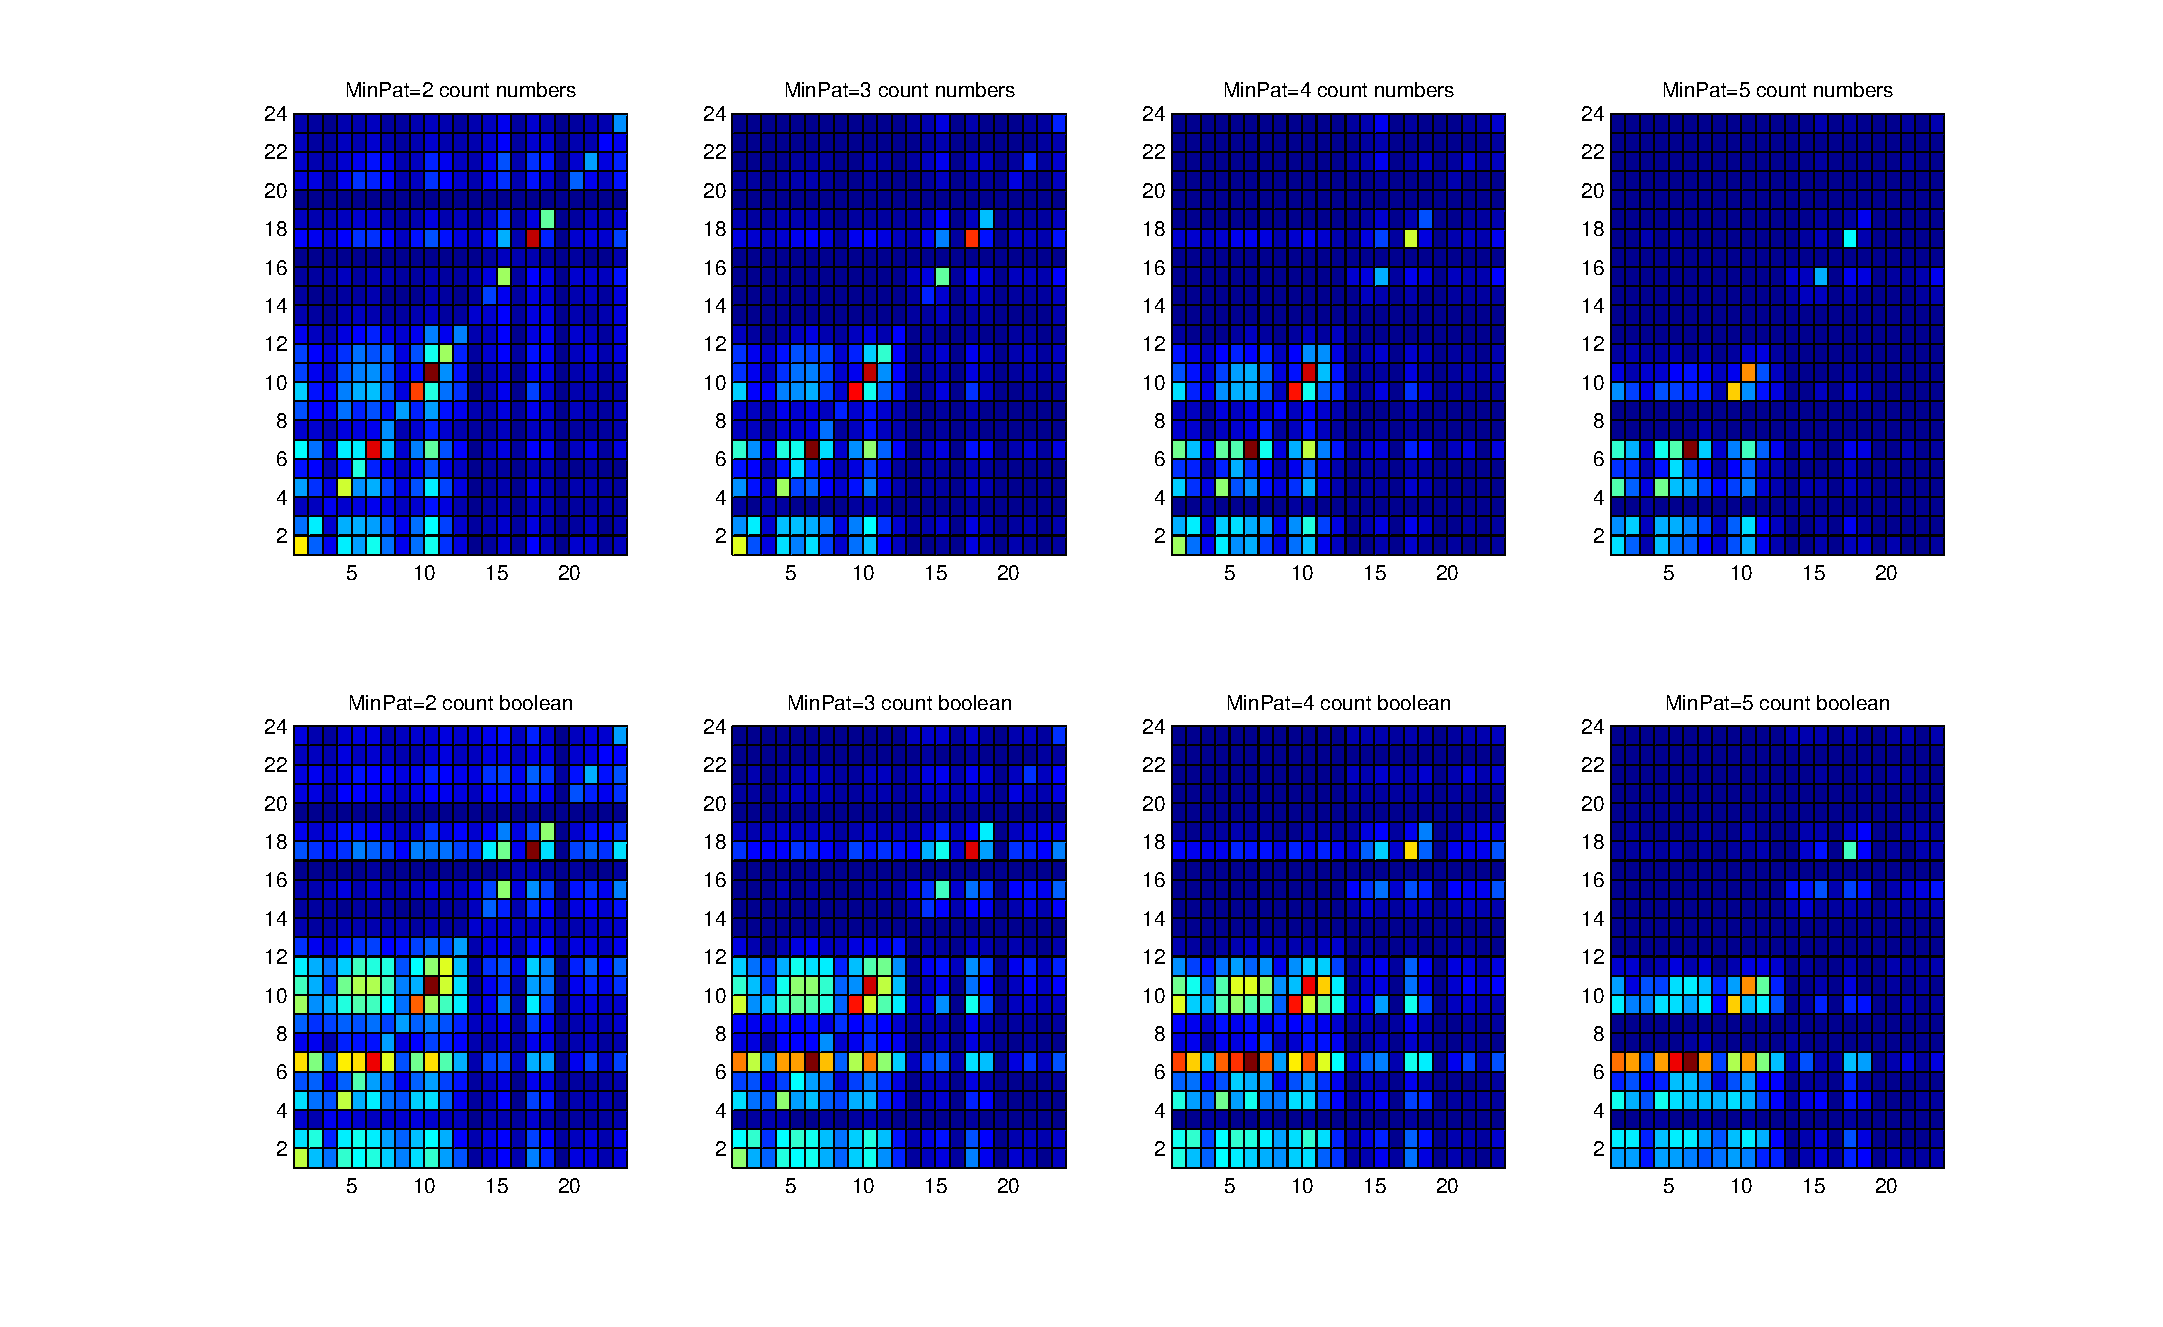
\includegraphics[width=173mm]{diff_metrics.eps}}
\caption{ Матчинги файлов для разных способов подсчета матчингов. Для каждого квадрата:первые 12 ячеек~--- контроль, вторые 12~--- без гиппокампа. 
По горизонтали откладывается из какого файла берутся паттерны, по вертикали откладывается в каком файле они ищутся. Т.о. правый нижний квадрант 
показывает <<какие паттерны нормальных мышей мы нашли у безгиппокампных>>, левый верхний квадрант говорит <<какие паттерны безгиппокампных
мышей мы наши у нормальных>>. Заметьте, что вообще говоря, здесь не должно быть симметрии, и это иногда можно наблюдать.
}
\end{figure}

\begin{figure}[h]
\noindent\centering{\includegraphics[width=173mm]{bcorr2.eps}}
\caption{ Более крупно для $MinPat=2$, boolean}

\end{figure}
\begin{figure}[h]
\noindent\centering{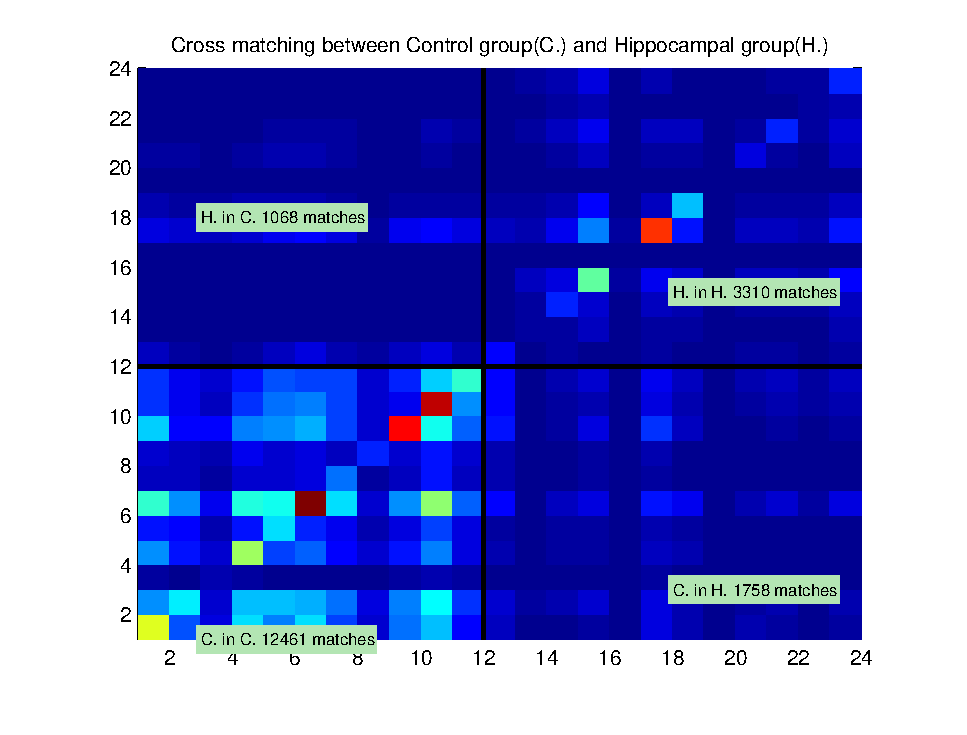
\includegraphics[width=173mm]{corr2.eps}}
\caption{ Более крупно для $MinPat=2$, frequent}

\end{figure}

\begin{figure}[h]
\noindent\centering{\includegraphics[width=173mm]{corr4.eps}}
\caption{ Более крупно для $MinPat=4$, frequent}
\end{figure}

Чисто визуально нравится больше всего случай $MinPat=2$+boolean(на практике он самый лучший, см. таблицу 1), так как в нем хорошо видны внутренние корреляции 
групп. Таким образом, действительно <<булевский>> матчинг более робастный, как и было написано в статье Ступа.
Отмечу, что двухвыборочный критерий Уилкоксона(ranksum) и двухвыборочный критерий Колмогорова Смирнова
хорошо срабатывают: группы левого нижнего и правого верхнего признаны взятыми из разных распределений. 
Подгруппы внутри этих квадрантов признаются взятыми из одного распределения при $p=0.01$.

\newpage~
\newpage~
\newpage
Теперь возьмем метод kNN и проведем схему leave-one-out. Т.е. берем для <<обучения>> 5 объектов из каждого класса
оставляем для теста по одному объекту из класса. Результаты для разным способов матчинга и значений $k$ в таблице.
\begin{table}
\centering{
\begin{tabular}{|c|c|c|c|c|c|c|c|c| }
\hline
~&1 & 2 & 3 & 4 &1b & 2b & 3b & 4b  \\[1ex]
\hline
$$k=1$$&58\% & 72\% & 71\% & 55\% & 87\% & 87\% & 84\% & 61\% \\ \hline
$$k=3$$&53\% & 59\% & 58\% & 56\% & 69\% & 73\% & 59\% & 49\% \\
\hline
\end{tabular}}
\caption{Процент правильных ответов классификации. Первые 4 колонки 
соответствуют частотному матчингу паттернов соответствующей минимальной длины(подсчет вхождений).
Вторые 4 колонки 
соответствуют булевскому матчингу паттернов соответствующей минимальной длины(подсчет фактов вхождения). Р-Паттерны}
\end{table}

Причем, мне кажется что результат не такой уж тривиальный. По гистограммам не так уж все ясно(самыне нижние рисунки). А матчинг 
Т-Пттернов дает результаты на порядок хуже.
Заметьте, что только, на рисунке~\ref{fig:TP} видная кое-какая связь и то
это связанно исключительно с тем, что данный контрольной группы длиннее, поэтому б\'{о}льшую
часть вносят короткие паттерны, которые находятся и в шуме. Ну а так как файлы контрольной
группы длиннее, то и матчингов этих больше. При других параметров выборки неотличимы, если
сравнивать Т-Паттерны. Качество классификации вообще никакое(см.табл. 2).

\begin{figure}[h]
\noindent\centering{\includegraphics[width=173mm]{tcorr1.eps}}
\caption{ Более крупно для $MinPat=2$, frequent. T-Паттерны}
\label{fig:TP}
\end{figure}
\begin{figure}[h]
\noindent\centering{\includegraphics[width=173mm]{tcorrb1.eps}}
\caption{ Более крупно для $MinPat=2$, boolean. T-Паттерны}

\end{figure}

\begin{figure}[h]
\noindent\centering{\includegraphics[width=173mm]{tcorrb2.eps}}
\caption{ Более крупно для $MinPat=4$, boolean. T-Паттерны}
\end{figure}

\begin{table}
\centering{
\begin{tabular}{|c|c|c|c|c|c|c| }
\hline
~&1 & 2 & 3 & 1b & 2b & 3b  \\[1ex]
\hline
$$k=1$$&46\% & 55\% & 50\% & 62\% & 51\% & 50\\ \hline
$$k=3$$&49\% & 69\% & 53\% & 67\% & 55\% & 50\% \\
\hline
\end{tabular}}
\caption{Процент правильных ответов классификации. Первые 3 колонки 
соответствуют частотному матчингу паттернов соответствующей минимальной длины(подсчет вхождений).
Вторые 3 колонки 
соответствуют булевскому матчингу паттернов соответствующей минимальной длины(подсчет фактов вхождения). Т-Паттерны.}
\end{table}

\begin{figure}[H]
	\begin{multicols}{2}
	\hfill
	\includegraphics[width=90mm]{hPC.eps}

	\includegraphics[width=90mm]{hPH.eps}
	\end{multicols}
	\caption{Гистограмма распределения длин P-Паттернов в контрольной группе(слева) и группе мышей без гиппокампа(справа).}
\end{figure}

\begin{figure}[H]
	\begin{multicols}{2}
	\hfill
	\includegraphics[width=90mm]{hTC.eps}

	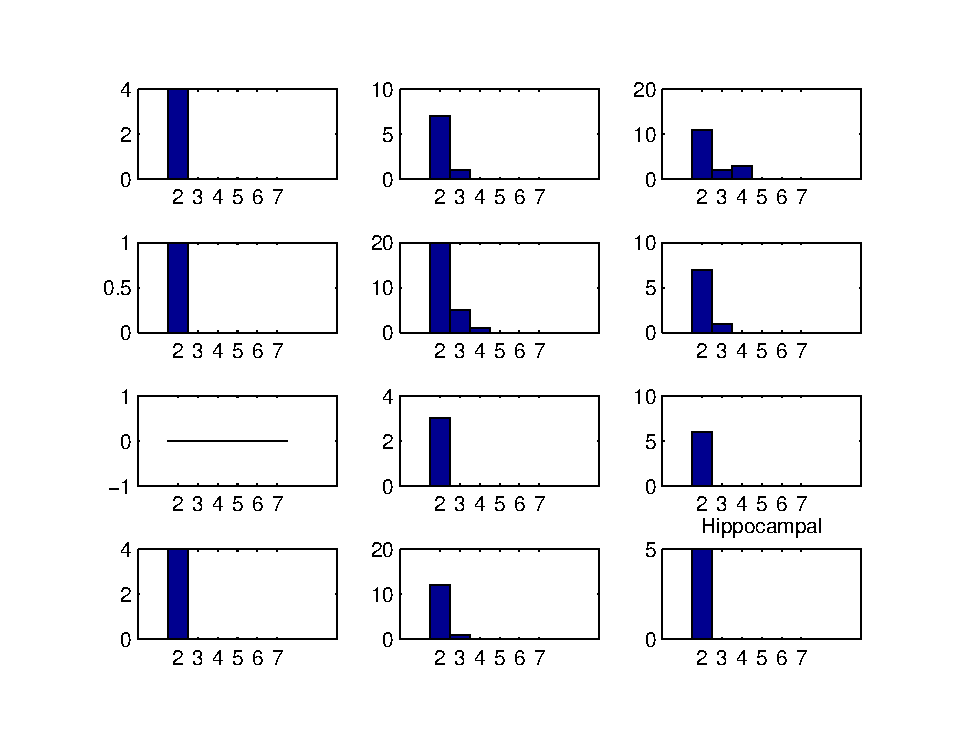
\includegraphics[width=90mm]{hTH.eps}
	\end{multicols}
	\caption{Гистограмма распределения длин Т-Паттернов в контрольной группе(слева) и группе мышей без гиппокампа(справа).}
\end{figure}


\newpage
\end{document}
